\documentclass{beamer}
\mode<presentation>
\usepackage{amsmath}
\usepackage{amssymb}
%\usepackage{advdate}
\usepackage{graphicx}
\usepackage{adjustbox}
\usepackage{subcaption}
\usepackage{enumitem}
\usepackage{multicol}
\usepackage{mathtools}
\usepackage{listings}
\usepackage{url}
\def\UrlBreaks{\do\/\do-}
\usetheme{Boadilla}
\usecolortheme{lily}
\setbeamertemplate{footline}
{
  \leavevmode%
  \hbox{%
  \begin{beamercolorbox}[wd=\paperwidth,ht=2.25ex,dp=1ex,right]{author in head/foot}%
    \insertframenumber{} / \inserttotalframenumber\hspace*{2ex} 
  \end{beamercolorbox}}%
  \vskip0pt%
}
\setbeamertemplate{navigation symbols}{}

\providecommand{\nCr}[2]{\,^{#1}C_{#2}} % nCr
\providecommand{\nPr}[2]{\,^{#1}P_{#2}} % nPr
\providecommand{\mbf}{\mathbf}
\providecommand{\pr}[1]{\ensuremath{\Pr\left(#1\right)}}
\providecommand{\qfunc}[1]{\ensuremath{Q\left(#1\right)}}
\providecommand{\sbrak}[1]{\ensuremath{{}\left[#1\right]}}
\providecommand{\lsbrak}[1]{\ensuremath{{}\left[#1\right.}}
\providecommand{\rsbrak}[1]{\ensuremath{{}\left.#1\right]}}
\providecommand{\brak}[1]{\ensuremath{\left(#1\right)}}
\providecommand{\lbrak}[1]{\ensuremath{\left(#1\right.}}
\providecommand{\rbrak}[1]{\ensuremath{\left.#1\right)}}
\providecommand{\cbrak}[1]{\ensuremath{\left\{#1\right\}}}
\providecommand{\lcbrak}[1]{\ensuremath{\left\{#1\right.}}
\providecommand{\rcbrak}[1]{\ensuremath{\left.#1\right\}}}
\theoremstyle{remark}
\newtheorem{rem}{Remark}
\newcommand{\sgn}{\mathop{\mathrm{sgn}}}
\providecommand{\abs}[1]{$\left\vert#1\right\vert$}
\providecommand{\res}[1]{\Res\displaylimits_{#1}} 
\providecommand{\norm}[1]{\lVert#1\rVert}
\providecommand{\mtx}[1]{\mathbf{#1}}
\providecommand{\mean}[1]{E$\left[ #1 \right]$}
\providecommand{\fourier}{\overset{\mathcal{F}}{ \rightleftharpoons}}
%\providecommand{\hilbert}{\overset{\mathcal{H}}{ \rightleftharpoons}}
\providecommand{\system}[1]{\overset{\mathcal{#1}}{ \longleftrightarrow}}
%\providecommand{\system}{\overset{\mathcal{H}}{ \longleftrightarrow}}
	%\newcommand{\solution}[2]{\textbf{Solution:}{#1}}
%\newcommand{\solution}{\noindent \textbf{Solution: }}
\providecommand{\dec}[2]{\ensuremath{\overset{#1}{\underset{#2}{\gtrless}}}}
\newcommand{\myvec}[1]{\ensuremath{\begin{pmatrix}#1\end{pmatrix}}}
\let\vec\mathbf

\lstset{
%language=C,
frame=single, 
breaklines=true,
columns=fullflexible
}

\numberwithin{equation}{section}

\title{4.4.20}
\author{AI25BTECH11024 - Pratyush Panda}
\begin{document}
\maketitle

\begin{frame}
\textbf{Question: } \\
The pair of linear equations $2x=5y+6$ and $15y=6x-18$ represents two lines which are: 
\begin{enumerate}
\item[(a)] intersecting
\item[(b)] parallel
\item[(c)] coincident
\item[(d)] either intersecting or parallel
\end{enumerate}
\end{frame}


\begin{frame}
\textbf{Solution: } \\
First, let us rewrite the equation of lines as;
\begin{align}
ax+by=c \\
2x-5y=6 \\
6x-15y=18 \textit{ or } 2x-5y=6
\end{align}

Normal vectors of the given lines can be written as:
\begin{align}
\Vec{n}=\myvec{a \\ b} \\
\Vec{n_1}=\myvec{2 \\ -5} && \Vec{n_2}=\myvec{2 \\ -5}
\end{align}
\end{frame}

\begin{frame}
Let the matrix $\Vec{M}$ be;
\begin{align}
\Vec{M}=\myvec{n_1 & n_2}^T=\myvec{2 & -5 \\ 2 & -5}
\end{align}

After reducing it to its Echelon form;
\begin{align}
\myvec{2 & -5 \\ 2 & -5}\xrightarrow{R_2\longleftrightarrow R_2-R_1}\myvec{2 & -5 \\ 0 & 0}
\end{align}

We can see that the rank of $\Vec{M}$ is 1. Therefore, the given lines can be either parallel or coincident.
\end{frame}

\begin{frame}
Now, consider the matrices $\Vec{P}$ and $\Vec{Q}$;
\begin{align}
\Vec{P}=\myvec{a_1 & c_1 \\ a_2 & c_2} && \Vec{Q}=\myvec{b_1 & c_1 \\ b_2 & c_2}
\end{align}
Since, the rank of both the matrices is 1. Thus, we can conclude that the the given lines are coincident.

\begin{figure}[H]
\centering
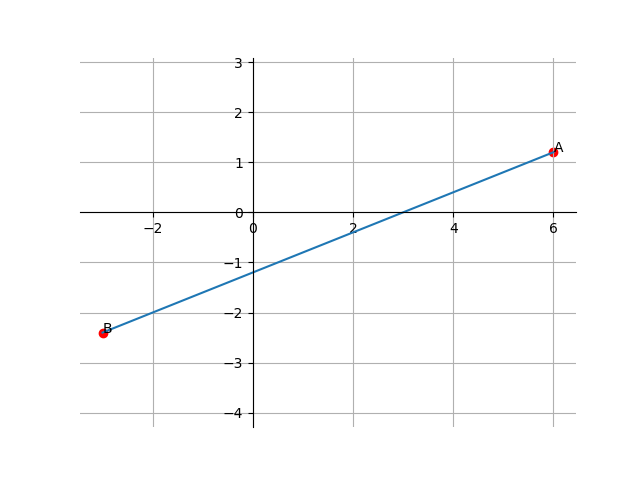
\includegraphics[width=0.6\columnwidth]{figs/img.png}
\caption*{}
\end{figure}
\end{frame}

\end{document}
